
\documentclass[letterpaper,hide notes,xcolor={table,svgnames},pdftex,10pt]{beamer}
\def\showexamples{t}

\usecolortheme{crane}
\setbeamertemplate{navigation symbols}{}

\usetheme{MyPittsburgh}
\usepackage{hyperref}
\usepackage{graphicx,xspace}
\usepackage[normalem]{ulem}
\usepackage{multicol}
\usepackage{amsmath,amssymb,amsthm,graphicx,xspace}
\newcommand\SF[1]{$\bigstar$\footnote{SF: #1}}

\usepackage[sfdefault,lf]{carlito}
\usepackage[T1]{fontenc}
\usepackage[scaled]{beramono}
\usepackage{tikzpagenodes}
\newcommand{\Rplus}{\protect\hspace{-.1em}\protect\raisebox{.35ex}{\small{\small\textbf{+}}}}
\newcommand{\Cpp}{\mbox{C\Rplus\Rplus}\xspace}

\newcounter{tmpnumSlide}
\newcounter{tmpnumNote}

\newcommand\mnote[1]{%
	\addtocounter{tmpnumSlide}{1}
	\ifdefined\showcues {~\tiny\fbox{\arabic{tmpnumSlide}}}\fi
	\note{\setlength{\parskip}{1ex}\addtocounter{tmpnumNote}{1}\textbf{\Large \arabic{tmpnumNote}:} {#1\par}}}

\newcommand\mmnote[1]{\note{\setlength{\parskip}{1ex}#1\par}}


\newcommand\mquestion[2]{{~\color{red}\fbox{?}}\note{\setlength{\parskip}{1ex}\par{\Large \textbf{?}} #1} \note{\setlength{\parskip}{1ex}\par{\Large \textbf{A}} #2\par}\ifdefined \presentationonly \pause \fi}

\newcommand\blackboard[1]{%
	\ifdefined   \showblackboard
		{#1}
	\else {\begin{center} \fbox{\colorbox{blue!30}{%
						\begin{minipage}{.95\linewidth}%
							\hspace{\stretch{1}} Some space intentionally left blank; done at the blackboard.%
						\end{minipage}}}\end{center}}%
	\fi%
}

\usepackage{listings}
\lstset{%
	keywordstyle=\bfseries,
	aboveskip=15pt,
	belowskip=15pt,
	captionpos=b,
	identifierstyle=\ttfamily,
	frame=lines,
	numbers=left, basicstyle=\scriptsize, numberstyle=\tiny, stepnumber=0, numbersep=2pt}

\usepackage{siunitx}
\newcommand\sius[1]{\num[group-separator = {,}]{#1}\si{\micro\second}}
\newcommand\sims[1]{\num[group-separator = {,}]{#1}\si{\milli\second}}
\newcommand\sins[1]{\num[group-separator = {,}]{#1}\si{\nano\second}}
\sisetup{group-separator = {,}, group-digits = true}

%% -------------------- tikz --------------------
\usepackage{tikz}
\usetikzlibrary{positioning}
\usetikzlibrary{arrows,backgrounds,automata,decorations.shapes,decorations.pathmorphing,decorations.markings,decorations.text}

\tikzstyle{place}=[circle,draw=blue!50,fill=blue!20,thick, inner sep=0pt,minimum size=6mm]
\tikzstyle{transition}=[rectangle,draw=black!50,fill=black!20,thick, inner sep=0pt,minimum size=4mm]

\tikzstyle{block}=[rectangle,draw=black, thick, inner sep=5pt]
\tikzstyle{bullet}=[circle,draw=black, fill=black, thin, inner sep=2pt]

\tikzstyle{pre}=[<-,shorten <=1pt,>=stealth',semithick]
\tikzstyle{post}=[->,shorten >=1pt,>=stealth',semithick]
\tikzstyle{bi}=[<->,shorten >=1pt,shorten <=1pt, >=stealth',semithick]

\tikzstyle{mut}=[-,>=stealth',semithick]

\tikzstyle{treereset}=[dashed,->, shorten >=1pt,>=stealth',thin]

\usepackage{ifmtarg}
\usepackage{xifthen}
\makeatletter
% new counter to now which frame it is within the sequence
\newcounter{multiframecounter}
% initialize buffer for previously used frame title
\gdef\lastframetitle{\textit{undefined}}
% new environment for a multi-frame
\newenvironment{multiframe}[1][]{%
	\ifthenelse{\isempty{#1}}{%
		% if no frame title was set via optional parameter,
		% only increase sequence counter by 1
		\addtocounter{multiframecounter}{1}%
	}{%
		% new frame title has been provided, thus
		% reset sequence counter to 1 and buffer frame title for later use
		\setcounter{multiframecounter}{1}%
		\gdef\lastframetitle{#1}%
	}%
	% start conventional frame environment and
	% automatically set frame title followed by sequence counter
	\begin{frame}%
		\frametitle{\lastframetitle~{\normalfont(\arabic{multiframecounter})}}%
		}{%
	\end{frame}%
}
\makeatother

\makeatletter
\newdimen\tu@tmpa%
\newdimen\ydiffl%
\newdimen\xdiffl%
\newcommand\ydiff[2]{%
	\coordinate (tmpnamea) at (#1);%
	\coordinate (tmpnameb) at (#2);%
	\pgfextracty{\tu@tmpa}{\pgfpointanchor{tmpnamea}{center}}%
	\pgfextracty{\ydiffl}{\pgfpointanchor{tmpnameb}{center}}%
	\advance\ydiffl by -\tu@tmpa%
}
\newcommand\xdiff[2]{%
	\coordinate (tmpnamea) at (#1);%
	\coordinate (tmpnameb) at (#2);%
	\pgfextractx{\tu@tmpa}{\pgfpointanchor{tmpnamea}{center}}%
	\pgfextractx{\xdiffl}{\pgfpointanchor{tmpnameb}{center}}%
	\advance\xdiffl by -\tu@tmpa%
}
\makeatother
\newcommand{\copyrightbox}[3][r]{%
	\begin{tikzpicture}%
		\node[inner sep=0pt,minimum size=2em](ciimage){#2};
		\usefont{OT1}{phv}{n}{n}\fontsize{4}{4}\selectfont
		\ydiff{ciimage.south}{ciimage.north}
		\xdiff{ciimage.west}{ciimage.east}
		\ifthenelse{\equal{#1}{r}}{%
			\node[inner sep=0pt,right=1ex of ciimage.south east,anchor=north west,rotate=90]%
			{\raggedleft\color{black!50}\parbox{\the\ydiffl}{\raggedright{}#3}};%
		}{%
			\ifthenelse{\equal{#1}{l}}{%
				\node[inner sep=0pt,right=1ex of ciimage.south west,anchor=south west,rotate=90]%
				{\raggedleft\color{black!50}\parbox{\the\ydiffl}{\raggedright{}#3}};%
			}{%
				\node[inner sep=0pt,below=1ex of ciimage.south west,anchor=north west]%
				{\raggedleft\color{black!50}\parbox{\the\xdiffl}{\raggedright{}#3}};%
			}
		}
	\end{tikzpicture}
}


%% --------------------

%\usepackage[excludeor]{everyhook}
%\PushPreHook{par}{\setbox0=\lastbox\llap{MUH}}\box0}

%\vspace*{\stretch{1}

%\setbox0=\lastbox \llap{\textbullet\enskip}\box0}

\setlength{\parskip}{\fill}

\newcommand\noskips{\setlength{\parskip}{1ex}}
\newcommand\doskips{\setlength{\parskip}{\fill}}

\newcommand\xx{\par\vspace*{\stretch{1}}\par}
\newcommand\xxs{\par\vspace*{2ex}\par}
\newcommand\tuple[1]{\langle #1 \rangle}
\newcommand\code[1]{{\sf \footnotesize #1}}
\newcommand\ex[1]{\uline{Example:} \ifdefined \presentationonly \pause \fi
	\ifdefined\showexamples#1\xspace\else{\uline{\hspace*{2cm}}}\fi}

\newcommand\ceil[1]{\lceil #1 \rceil}


\AtBeginSection[]
{
	\begin{frame}
		\frametitle{Outline}
		\tableofcontents[currentsection]
	\end{frame}
}



\pgfdeclarelayer{edgelayer}
\pgfdeclarelayer{nodelayer}
\pgfsetlayers{edgelayer,nodelayer,main}

\tikzstyle{none}=[inner sep=0pt]
\tikzstyle{rn}=[circle,fill=Red,draw=Black,line width=0.8 pt]
\tikzstyle{gn}=[circle,fill=Lime,draw=Black,line width=0.8 pt]
\tikzstyle{yn}=[circle,fill=Yellow,draw=Black,line width=0.8 pt]
\tikzstyle{empty}=[circle,fill=White,draw=Black]
\tikzstyle{bw} = [rectangle, draw, fill=blue!20,
text width=4em, text centered, rounded corners, minimum height=2em]

\newcommand{\CcNote}[1]{% longname
	This work is licensed under the \textit{Creative Commons #1 3.0 License}.%
}
\newcommand{\CcImageBy}[1]{%
	\includegraphics[scale=#1]{creative_commons/cc_by_30.pdf}%
}
\newcommand{\CcImageSa}[1]{%
	\includegraphics[scale=#1]{creative_commons/cc_sa_30.pdf}%
}
\newcommand{\CcImageNc}[1]{%
	\includegraphics[scale=#1]{creative_commons/cc_nc_30.pdf}%
}
\newcommand{\CcGroupBySa}[2]{% zoom, gap
	\CcImageBy{#1}\hspace*{#2}\CcImageNc{#1}\hspace*{#2}\CcImageSa{#1}%
}
\newcommand{\CcLongnameByNcSa}{Attribution-NonCommercial-ShareAlike}

\newenvironment{changemargin}[1]{% 
	\begin{list}{}{% 
		\setlength{\topsep}{0pt}% 
		\setlength{\leftmargin}{#1}% 
		\setlength{\rightmargin}{1em}
		\setlength{\listparindent}{\parindent}% 
		\setlength{\itemindent}{\parindent}% 
		      \setlength{\parsep}{\parskip}% 
		      }% 
		\item[]}{\end{list}}




\title{Lecture 19 --- Scheduling: Idling, Priorities, Multiprocessor }

\author{Jeff Zarnett \\ \small \texttt{jzarnett@uwaterloo.ca}}
\institute{Department of Electrical and Computer Engineering \\
  University of Waterloo}
\date{\today}


\begin{document}

\begin{frame}
  \titlepage

 \end{frame}



\begin{frame}
\frametitle{Scheduling Algorithms, Continued}

\begin{center}
	
\includegraphics[width=0.3\textwidth]{images/theresmore.jpg}
\end{center}

Carrying on from last time, we will examine some more scheduling algorithms.

\end{frame}

\begin{frame}
\frametitle{Highest Response Ratio Next}

\begin{center}
	
\includegraphics[width=0.8\textwidth]{images/responsive.jpg}
\end{center}

\end{frame}

\begin{frame}
\frametitle{Highest Response Ratio Next}

We will introduce a new measure: \alert{normalized turnaround time}. 

This is the ratio of the turnaround time (the time waiting plus the amount of time taken to execute) to the service time (the time it takes to execute). 

We can tolerate longer processes waiting a comparatively longer period of time. 

\end{frame}

\begin{frame}
\frametitle{Highest Response Ratio Next}

Goal: minimize not only the normalized turnaround time for each process, but to minimize the average over all processes.


\end{frame}

\begin{frame}
\frametitle{HRRN}

Calculate $R = \frac{w + s}{s}$ 
where $w$ is the waiting time and $s$ is the service time. 

The service time is, as always, a guess. 

When it is time to select the next process to run, choose the process with the highest $R$ value. 

A new process will have a value of 1.0 at the beginning, because it has spent no time waiting (yet). Thus it is not that likely to get selected.


\end{frame}

\begin{frame}
\frametitle{HRRN}

Jobs with a small $s$, i.e., short jobs, are likely to get scheduled quickly. 

The HRRN approach introduces something important: age of the process. 

\end{frame}

\begin{frame}
\frametitle{HRRN}

A process that has spent a long time waiting rises in priority until it gets a turn. 

So processes will not starve, because even a process that is expected to have a very long $s$ will eventually have a high enough $R$ due to the growth of $w$.

We still need to estimate $s$, which may or may not be simple guessing. 


\end{frame}

\begin{frame}
\frametitle{Multilevel Queue (Feedback)}

\begin{center}
	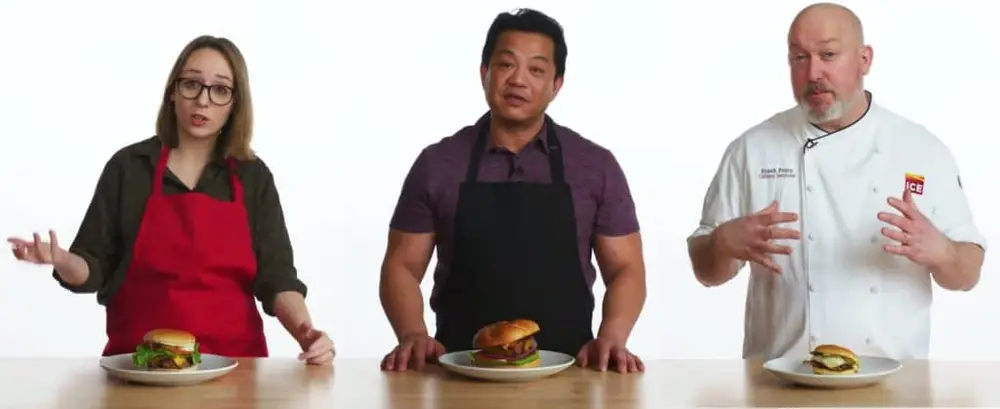
\includegraphics[width=0.6\textwidth]{images/levels1.jpg}
	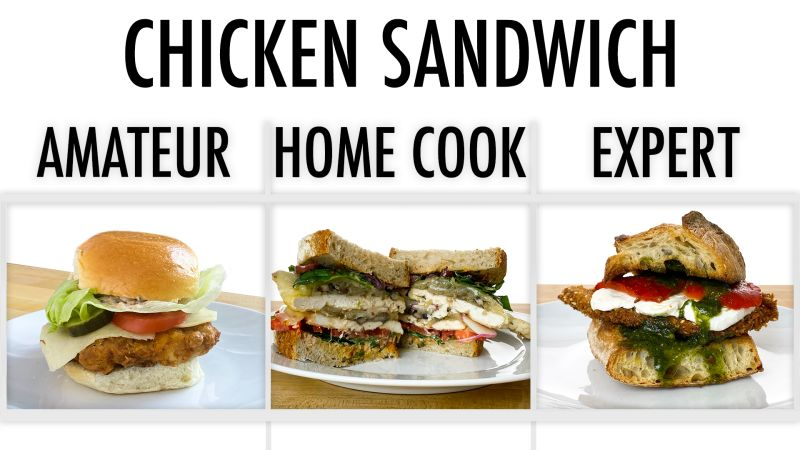
\includegraphics[width=0.6\textwidth]{images/levels2.jpg}
\end{center}


\end{frame}

\begin{frame}
\frametitle{Multilevel Queue (Feedback)}

For the most part, until now, we have treated processes more or less equally (except when we have taken the highest priority process). 

While it might seem very fair, it may not be ideal for a situation where processes behave differently. 

\end{frame}

\begin{frame}
\frametitle{Multilevel Queue (Feedback)}

A desktop or laptop has many processes running (foreground/background). 

We can apply different scheduling algorithms to different types of process.

\end{frame}

\begin{frame}
\frametitle{Multilevel Queue (Feedback)}

The multilevel queue takes the ready queue and breaks it up into several. 

A process can be in one (but only one) of the queues. 

It is assigned to the queue based on some attribute of the process (priority, memory needs, foreground/background, et cetera). 


\end{frame}

\begin{frame}
\frametitle{Multilevel Queue (Feedback)}

\begin{center}
	
\includegraphics[width=\textwidth]{images/choice-sweat.jpg}
\end{center}

The foreground queue, for example, could be scheduled by Round Robin, and the background by First-Come, First-Served.


\end{frame}

\begin{frame}
\frametitle{Multilevel Queue (Feedback)}

When there are multiple queues, we also need a way of choosing which of the queues to take from next. 

We might say some queues have absolute priority over others, or we might have time slicing amongst the queues. 

This could be balanced evenly (rotate through each) or give more time slices to some queues at the expense of others.

\end{frame}

\begin{frame}
\frametitle{MLQ Example: CTSS}

An example of this was the Compatible TimeSharing System on the IBM~7094. 

Give CPU-Bound processes longer blocks of time to execute so they would not have to spend so much time swapping. 

In the highest priority class, a process got 1 time slice; in the next one down, a process got 2 time slices; the third class meant 4 time slices, and so on. 

\end{frame}

\begin{frame}
\frametitle{MLQ Example: CTSS}

If a process ran up against the limit of a time slice it was moved down a class. 

So it got a lower priority, but when it did get selected to run, it was able to run with a lower chance of being interrupted.


\end{frame}

\begin{frame}
\frametitle{CTSS: Ratchet}

Like a few schemes we have seen so far, this is a ratchet. 

A process can move down in the priority list, but there does not appear to be a way for it to move up. 

A process that needed a lot of CPU early on was going to be punished ``forever''.


\end{frame}

\begin{frame}
\frametitle{CTSS: Meddling Users}

If the user pressed the Enter key, it might be a sign the process was likely to become interactive (and therefore should move up in priority). 

Some genius user (there's always one), figured out that by pressing the enter button repeatedly, his long running processes would finish faster. 

\begin{center}
	
\includegraphics[width=0.4\textwidth]{images/meddling.jpg}
\end{center}

\end{frame}

\begin{frame}
\frametitle{CTSS: Meddling Users}

This was a bit unfair; his processes got priority over the others. 

Things really broke down when this individual decided to be nice:\\
\quad ... He told all his friends. 

Suddenly everyone was doing it and the benefit of the system was lost.


\end{frame}

\begin{frame}
\frametitle{MLQ/Feedback}

This scheduling algorithm may also be referred to as \alert{feedback}. 

We do not have any information in advance about how long processes will be. 

Assign priority based on the amount of CPU time assigned so far. 

A process that has used a lot of CPU so far gets lower priority.


\end{frame}

\begin{frame}
\frametitle{Guaranteed Scheduling}

\begin{center}
	
\includegraphics[width=\textwidth]{images/guarantee.jpg}
\end{center}

\end{frame}

\begin{frame}
\frametitle{Guaranteed Scheduling}

Promise the users something and then fulfill that promise. 

If there are $n$ users, each gets an equal share (1/$n$) of the CPU time. 

Or with $m$ processes, each process gets 1/$m$ of the CPU time.


\end{frame}

\begin{frame}
\frametitle{Guaranteed Scheduling}

The system must keep track of how much CPU time each process has received. 

It then considers the how this value compares to the ideal. 

If a process has a value of 0.5, it had only half the CPU it ``should'' have received. 

If it has a value of 2.0, it has had double. 

So the scheduling algorithm is then to run the process with the lowest score, trying to keep all values as close to 1.0 as we can

\end{frame}

\begin{frame}
\frametitle{Lottery}

The lottery is a system to give predictable results with a simple implementation. 

\begin{center}
	
\includegraphics[width=0.5\textwidth]{images/lottery.jpg}
\end{center}

\end{frame}

\begin{frame}
\frametitle{Lottery}

The premise is that every process gets some number of ``lottery tickets'' for each resource (e.g., CPU). 

When a decision has to be made, a lottery ticket is selected at random. 

The process that holds that ticket gets that resource.

\end{frame}

\begin{frame}
\frametitle{Lottery}

This system provides clarity; if a process has priority $p$, what does that mean? 

If a process has a fraction $f$ of the total tickets, then we can expect that process to get about $f$\% of the resource. 

When a process is created or terminates this may increase or decrease the number of tickets, or result in their redistribution.


\end{frame}

\begin{frame}
\frametitle{Lottery}

More important processes get more tickets \& have a higher chance of winning. 

If there are 100 tickets outstanding, if a process has 25 of them, it has a 25\% chance of winning any given draw. 

To increase a process's chance of winning, give it more tickets.\\
\quad To decrease it, give it fewer. 

Unlike in the real lottery, though, there is always a winner.

\end{frame}

\begin{frame}
\frametitle{Lottery}

Co-operating processes may be permitted to exchange tickets. 

A client that sends a request to a server might then give its tickets to the server.

This increases the chance the server gets the resources to run next and respond.

\end{frame}

\begin{frame}
\frametitle{Lottery}

This is a lot less overhead than guaranteed scheduling. 

We do not keep track of how much of the resource a process has received. 

Assuming that the lottery system is sufficiently random, over time the resource allocation will tend towards the proportions of the tickets each process holds. 

If process $A$ has 20\% of the tickets, $B$ has 30\%, and $C$ has 50\%, then the CPU will be given to the processes in approximately a 20:30:50 ratio, as expected.


\end{frame}

\begin{frame}
\frametitle{The Idle Task}

Sometimes our scheduling algorithm cannot produce a new process to run next because there is, quite frankly, nothing to do. 

\begin{center}
	
\includegraphics[width= \textwidth]{images/bored.jpg}
\end{center}

The actual implementation of the idle thread may vary across different systems. 

\end{frame}

\begin{frame}
\frametitle{The Idle Task}

In some cases it is just repeatedly invoking the scheduler.\\
\quad In others it does a bit of useless addition.\\
\quad Or it might just be a whole bunch of \texttt{NOP} instructions. 

The CPU can be told to halt/switch to a low power state. 

Whatever it actually ``does'', the idle thread never has any dependencies on anything else and is always ready to run.

\end{frame}

\begin{frame}
\frametitle{The Idle Task}

Since the idle task does not necessarily do much, why have it? 

\end{frame}

\begin{frame}
\frametitle{The Idle Task}

It prevents having special cases in the scheduler, first of all. 

It also provides accounting information about how much of the time the CPU is not doing anything. 

In fact, a lot of the time on the desktop or laptop, task manager will tell you that ``System Idle Process'' is taking up a large percentage of the CPU. 

You will recognize that this just means the CPU is not doing anything;\\
\quad It does not mean that some system process is using up all your CPU's time.


\end{frame}

\begin{frame}
\frametitle{Making Use of The Time}

Saving power by shutting down (parts of) the processor seems like a nice savings of energy (and potentially increases battery life). 

But: time when the CPU is doing nothing might potentially be put to use.

\end{frame}

\begin{frame}
\frametitle{Making Use of The Time}


There are usually some accounting and housekeeping tasks that the CPU can be doing when it has nothing else. 
 
For example, the OS could collect statistical data, or defragment the hard drive.


\end{frame}

\begin{frame}
\frametitle{Bumping the Priority}

Sometimes we get into a situation called a \alert{priority inversion}. 

\begin{center}
	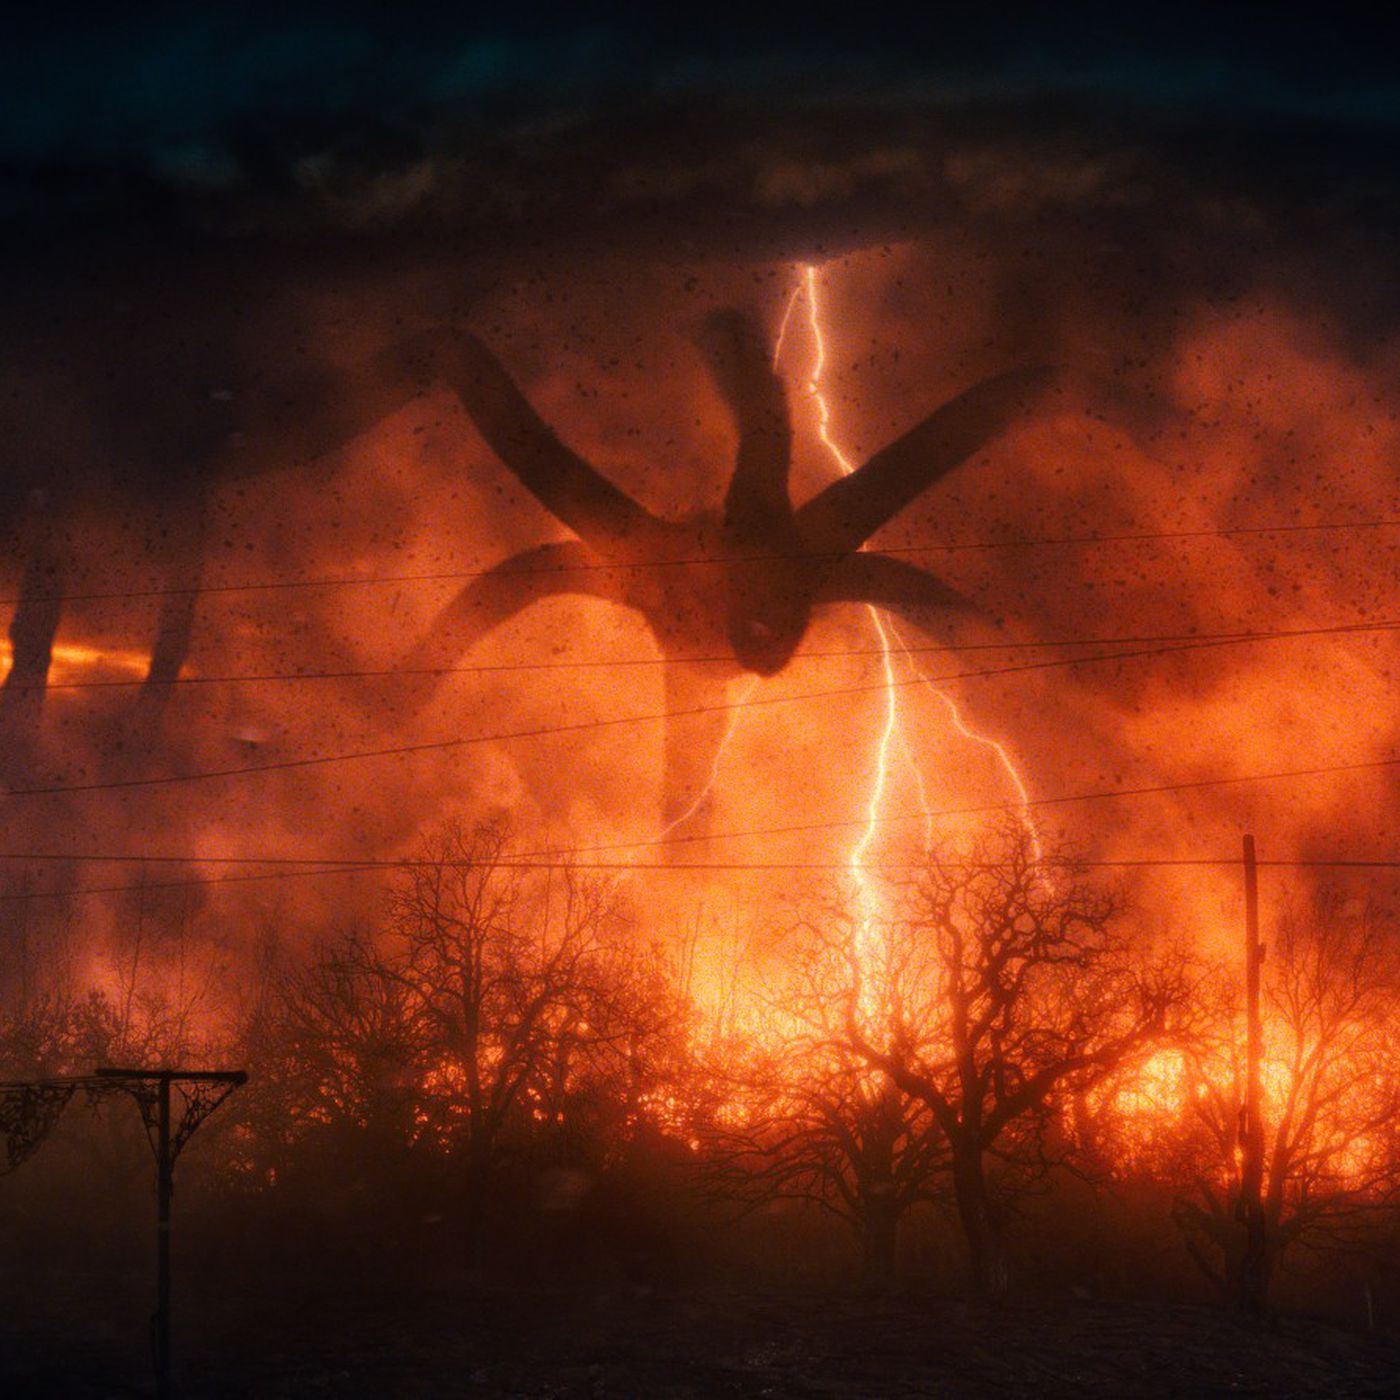
\includegraphics[width=0.6\textwidth]{images/upsidedown.jpg}
\end{center}

\end{frame}

\begin{frame}
\frametitle{Bumping the Priority}


A high priority process is waiting for a low priority process. 

$P_{1}$ is high priority and is blocked on a semaphore, while $P_{2}$ is in a critical section. 

As $P_{2}$ is low priority, it might be a long time before $P_{2}$ is selected again to run and can finish and exit the critical section. 

\end{frame}

\begin{frame}
\frametitle{Priority Inversion}

$P_{1}$ cannot run, because it is blocked, and it could be blocked for a long time. 

In the meantime, other processes with lower priority than $P_{1}$ (but higher than $P_{2}$) carry on execution. 

Having $P_{1}$ waiting for the lower priority processes is rather undesirable.


\end{frame}

\begin{frame}
\frametitle{Priority Inheritance}

The solution is \alert{priority inheritance}. 

The right thing to do is to bump up the priority of $P_{2}$, temporarily, to be equal to that of $P_{1}$, so that $P_{1}$ can be unblocked as quickly as possible. 

To generalize, a lower priority process should inherit the higher priority if a higher priority process is waiting for a resource the lower priority process holds. 

So $P_{2}$ will get selected, will execute and exit the critical section. 

Its priority then falls, meaning $P_{1}$ will be selected and may continue.

\end{frame}

\begin{frame}
\frametitle{Priority Inheritance}

A famous case of priority inversion took place on the Mars Pathfinder rover.

\begin{center}
	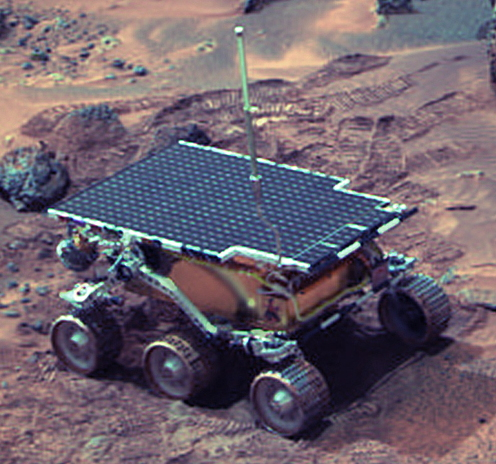
\includegraphics[width=0.5\textwidth]{images/pathfinder.jpg}
\end{center}

The solution was to enable priority inheritance.

\end{frame}

\begin{frame}
\frametitle{Multiprocessor Scheduling}

If you thought scheduling for a single processor was complicated enough, well, things are about to get exponentially harder. 

When we have more than one processor working on things at a time, then the complexity increases dramatically. 


\end{frame}

\begin{frame}
\frametitle{Multiprocessor Systems}

We can classify multiprocessor systems into three major buckets:

\begin{enumerate}
	\item \textbf{Distributed}.
	\item \textbf{Functionally Specialized}.
	\item \textbf{Tightly Coupled}.
\end{enumerate}

The third is our focus here.

\end{frame}

\begin{frame}
\frametitle{Multiprocessor: Granularity}

Then we have to worry about the interactions of various processes.

Specifically, how often they plan to interact.

\begin{center}
\begin{tabular}{l|l|l}
	\textbf{Grain Size} & \textbf{Description} & \textbf{Interval (Instructions)}\\ \hline
	Fine & Single instruction stream & $< 20$ \\\hline
	Medium & Single application & $20 - 200$ \\\hline
	Coarse & Multiple processes & $200 - 2000$ \\\hline
	Very Coarse & Distributed computing & $2000 - 1$M \\\hline
	Independent & Unrelated processes & N/A \\

\end{tabular}
\end{center}

\end{frame}

\begin{frame}
\frametitle{Granularity}

The finer-grained the parallelism, the more care and attention needs to be given to how we are going to schedule a process in a multiprocessor system. 

If the processes are independent, then there is not too much to worry about. 

If we are taking a single process's thread and doing different instructions on different CPUs, then we have to be very careful.

\end{frame}

\begin{frame}
\frametitle{Asymmetric vs Symmetric}
Asymmetric multiprocessing: a boss processor and this one alone is responsible for assigning work and managing the kernel data structures. 

Symmetric multiprocessing, each processor is responsible for scheduling itself. 

We will need to make use of mutual exclusion and other synchronization techniques in the kernel to prevent errors.

We do not want to have two processors trying to dequeue from the ready queue at the same time, after all.

\end{frame}

\begin{frame}
\frametitle{Processor Affinity}

Imagine that every processor has its own cache (e.g., the L1, L2, \& L3 caches).

We want to have \alert{processor affinity}. 

A process will have a bunch of its data in the cache of that processor. 

If the process begins executing on another processor, all the data is in the ``wrong'' cache and there will be a lot more cache misses. 

This desire to stick with a certain processor is called processor affinity.


\end{frame}

\begin{frame}
\frametitle{Processor Affinity}

If the OS is just going to make an effort but not guarantee that a process runs on a given processor, that is called \alert{soft affinity}. 

A process can move from one processor to another, but will not do so if it can avoid it. 

The alternative is \alert{hard affinity}: a process will only run on a specified processor (or set of processors). 

Linux, for example, has both soft and hard affinity

\end{frame}

\begin{frame}
\frametitle{Affinity - NUMA}

For the most part any memory read takes as much time as any other. 

One bus connecting the CPU to all of main memory? That is a safe assumption.

  If the CPU can access some parts of memory faster than others, the system has \alert{non-uniform memory access} (NUMA).

\end{frame}

\begin{frame}
\frametitle{NUMA}

\begin{center}
	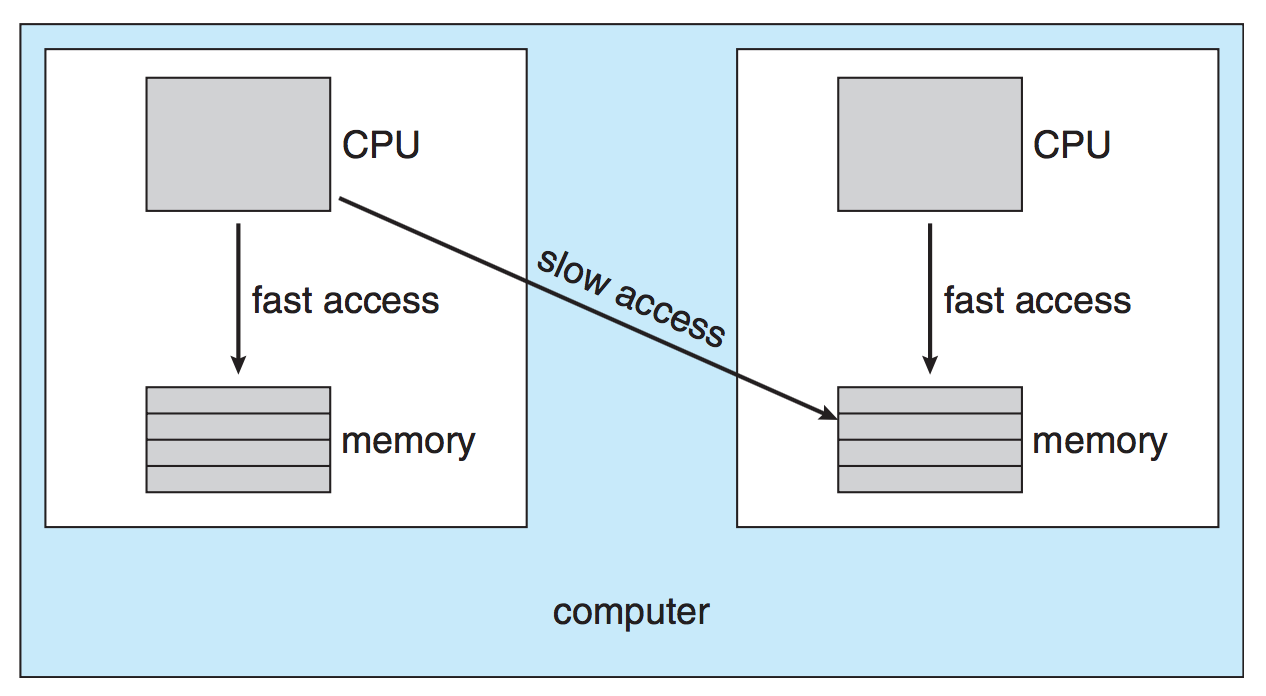
\includegraphics[width=0.85\textwidth]{images/numa.png}
\end{center}

\end{frame}

\begin{frame}
\frametitle{NUMA}

With NUMA: choice of processor should be based on where the memory of the process is located.

The memory allocation routine should also pay attention to where to allocate memory requests.
  
If there is data in one of the other blocks of memory, it does not mean game over, but it means slower execution.

\end{frame}

\begin{frame}
\frametitle{Load Balancing}

If we have 4 processors, it is less than ideal to have one processor at 100\% utilization and 3 processors sitting around doing nothing. 

We want to keep the workload balanced between all the different systems. 

The process for this is \alert{load balancing}.

\end{frame}

\begin{frame}
\frametitle{Load Balancing}

Load balancing is typically necessary only where each processor has its own private queue of processes to run. 

If there is a common ready queue then load balancing will tend to happen all on its own.

A processor with nothing to do will simply take the next process from the queue. 

But in most of the modern operating systems we are familiar with, each processor does have a private queue, so we need to do load balancing.

\end{frame}

\begin{frame}
\frametitle{Push and Pull Load Balancing}

There are two, non-exclusive approaches: \alert{push} and \alert{pull} migration. 


Push migration: a task periodically checks how busy each processor is and then moves processes around to balance things out (to within some tolerance). 

Pull migration: a processor with nothing to do ``steals'' a process from the queue of a busy processor. 

The Linux and FreeBSD schedulers, for example, use both.

\end{frame}

\begin{frame}
\frametitle{Balancing Affinity}

Load balancing sometimes conflicts with processor affinity. 

If a process has a hard affinity for a processor, it cannot be migrated. 

If there is a soft affinity, it can be moved, but it is not our first choice.

\end{frame}

\begin{frame}
\frametitle{Balancing Affinity}

Should we always move a process despite the fact that it means a whole bunch of cache misses?

Should we never do so and leave processors idle? 

Perhaps the best thing to do is to put a certain ``penalty'' on moving.

Only move a process from one queue to another if it would be worthwhile (i.e., the imbalance is sufficiently large).

\end{frame}

\begin{frame}
\frametitle{Multicore Processors}

Before the early 2000s, the only way to get multiple processors in the system was to have multiple physical chips. 

If you open up your laptop you are likely to find one physical chip. 

What gives? \alert{Multicore processors}. 

As far as the operating system is concerned, a quad-core chip is made of four logical processors.

\end{frame}

\begin{frame}
\frametitle{Multicore Processors}

On a cache miss the CPU core can spend a lot of time (50\%?) of its time waiting for that read to take place.

  We might refer to periods of time where there is computation as a compute cycle, and time spent waiting for memory as a \alert{memory stall}. 
  
  These tend to alternate, though the length of time for each will vary. 
  
  A question of how often memory is accessed and how many cache misses.

\end{frame}

\begin{frame}
\frametitle{Compute Cycles and Memory Stalls}

\begin{center}
	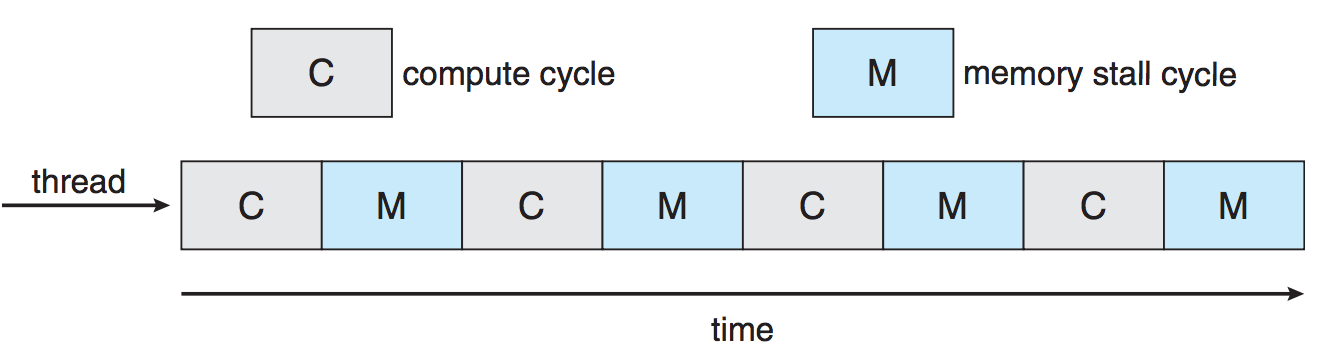
\includegraphics[width=\textwidth]{images/memory-stall.png}
\end{center}

\end{frame}

\begin{frame}
\frametitle{Memory Stall}

During a memory stall, the processor core may have nothing to do. 

You can sometimes move instructions around so that the memory read goes out ``early''.

A few other instructions can be executed in the meantime. 

(Take CPU design / programming for performance classes.)

\end{frame}

\begin{frame}
\frametitle{Hyperthreading}

To offset this problem, the solution was originally called \alert{hyperthreading}.

Two threads are assigned to each core; if one thread does a memory access or stalls, the code can switch to another thread with a limited penalty. 

\end{frame}

\begin{frame}
\frametitle{Hyperthreading}

\begin{center}
	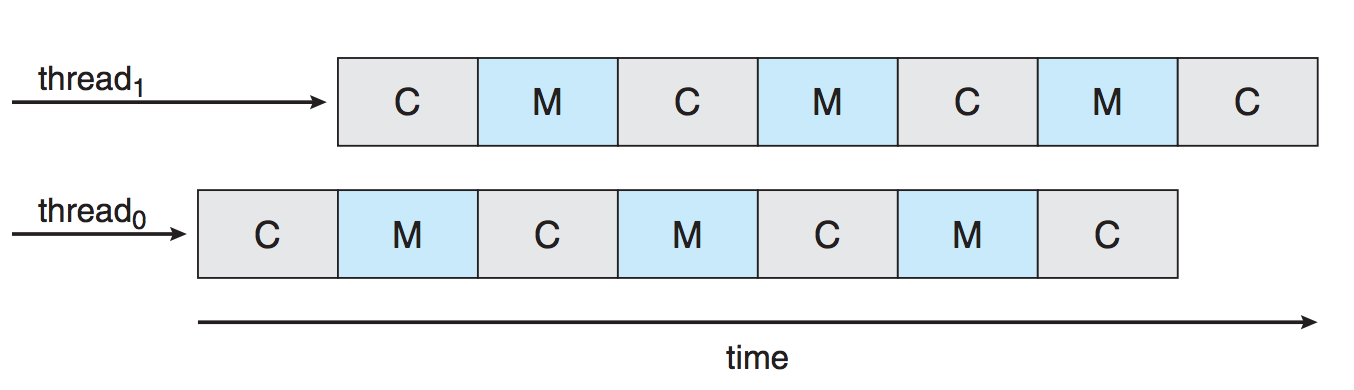
\includegraphics[width=\textwidth]{images/hyperthreading.png}
\end{center}

\end{frame}

\begin{frame}
\frametitle{Hyper- and Multithreading}

Coarse-grained multithreading: flushing the instruction pipeline. 

That is expensive. 

Fine-grained multithreading: alternation between 2 threads in the pipeline. 

The cost of switching between these two threads is small.

\end{frame}

\begin{frame}
\frametitle{Two Levels of Scheduling}

So now we have two different levels of scheduling.

1. Assigning a process or thread to a processor (job of the operating system)

2. When to swap between the two threads in the core (job of the hardware). 

\end{frame}


\end{document}

